\documentclass[10pt]{article}

\usepackage[margin=1in, letterpaper]{geometry}
\usepackage{parskip}

\usepackage{amsthm, amsmath, amssymb}
\usepackage{gensymb}  % For use of degree symbol
\usepackage[pdftex]{graphicx}
\usepackage{hyperref}

\usepackage{enumerate} % For use of (a), (b), et cetera
\usepackage{booktabs} % Tables
\usepackage[margin=20pt, labelfont=bf, labelsep=period,
justification=justified]{caption} % Captions in figure floats

% ======================
% Document setup, layout
% ======================

% The following metadata will show up in the PDF properties
\hypersetup{
	colorlinks = true,
	urlcolor = magenta,  % Links to URLs
	linkcolor = blue,  % Links within PDF
	pdfauthor = {Aaron Tran},
	pdfkeywords = {berkeley},
	pdftitle = {Astro 121, UG Radio Lab, Lab 4 - \today},
	pdfsubject = {},
	pdfpagemode = UseNone
}

% Don't indent paragraphs
\setlength\parindent{0em}

% Slightly more compact lines
\linespread{0.95}

% ===============
% Useful commands
% ===============
\newcommand {\mt}{\mathrm}
\newcommand {\unit}[1]{\; \mt{#1}}
% http://vemod.net/typesetting-units-in-latex

% Sets, operators
\newcommand {\ints}{\mathbb{Z}}
\newcommand {\ptl}{\partial}
\newcommand {\dl}{\nabla}

\begin{document}

% =======
% Titling
% =======
\begin{center}
\Large{Partial $1420\unit{MHz}$ HI Survey of the North Polar Spur}

\normalsize
\textbf{Aaron Tran}${}^{1,3}$ \\
Isaac A. Domagalski${}^{1,2}$, Caleb Levy${}^{1,2}$ \\
Aaron Parsons${}^{2,4,5}$, Garrett K. Keating${}^{2,4,5}$, Baylee Bordwell${}^{2,5}$ \\
\footnotesize
${}^1$Central Intelligence Agency, 1000 Colonial Farm Rd, McLean, VA 22101, USA \\
${}^2$Dept. Astronomy, UC Berkeley, D-23 Hearst Field Annex, Berkeley, CA 94720, USA \\
${}^3$Dept. Earth and Planetary Science, UC Berkeley, 335 McCone Hall, Berkeley, CA 94720, USA \\
${}^4$Radio Astronomy Laboratory, UC Berkeley, Berkeley, CA 94720, USA \\
${}^5$Undergraduate Radio Laboratory teaching staff \\
\textit{Received in incomplete form 2014 May 6, revised 2014 May ?!}
\end{center}

% ========
% Abstract
% ========
\section*{Abstract}

We observe the north polar spur and stuff

% ============
% Introduction
% ============
\section{Introduction}

background on NPS.  Supernovae, snowploughs, shocks, Sedov, whatever.
ISM, physical properties inferable.

The North Polar Spur is a prominent ridge structure within the greater Loop-I region which emits continuum and HI line emission at $1420 \unit{MHz}$ [\textit{Heiles et al.}, 1980]

% ============
% Observations
% ============
\section{Observations}

% ------------------------
% Leuschner specifications
% ------------------------
\subsection{Leuschner radio dish}

We use the Leuschner radio dish ($37\degree 55' 10.2'' \unit{N}$, $-122\degree 09' 12.4'' \unit{E}$), operated by UC Berkeley as part of Leuschner Observatory, to collect single-dish observations of the hyperfine HI line.  The Leuschner radio dish, hereafter Leuschner (Figure \ref{fig:kartp}), has diameter $3.6\unit{m}$ or $4.5\unit{m}$ depending on who is asked; the beamwidth is $\sim4\degree$ at its operating frequency of $1420 \unit{MHz}$.  Leuschner's view at low altitudes is blocked by surrounding hills; to the north Leuschner may point above $\sim50\degree$, to the south Leuschner may point to $20$--$30\degree$ altitude.  The Leuschner radio dish was originally built for the SETI Rapid Prototype Array near Leuschner Observatory, an early prototype for the now-underfunded and incomplete Allen Telescope Array.  The dish has since been appropriated for undergraduate education; its sibling dishes have been dismantled or turned into gigantic bats (e.g., \href{http://patriciavader.com/artwork/1696610\_The\_Giant\_Bat.html}{http://patriciavader.com/artwork/1696610\_The\_Giant\_Bat.html}).

\begin{figure}[!ht]
    \centering
    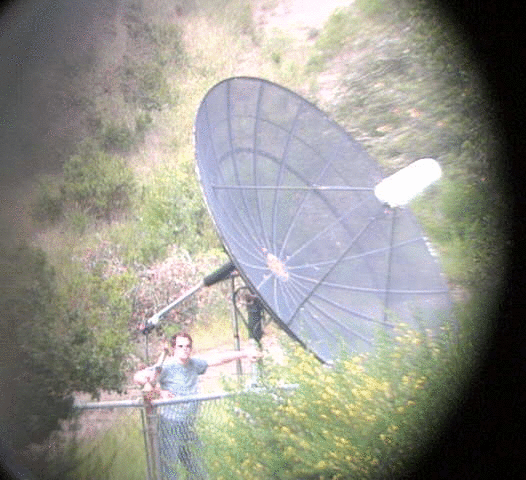
\includegraphics[width=0.5\textwidth]{kartp.png} \\
    \caption{The Leuschner dish has beamwidth $\sim 4 \degree$ at $1420 \unit{MHz}$.  Here the dish is shown with its erstwhile caretaker, \emph{kartp} (courtesy of I. Domagalski, E. Herrera, K. Moses).}
    \label{fig:kartp}
\end{figure}

RF waves incident on Leuschner are passed through a $200 \unit{MHz}$ bandpass filter centered on $1420 \unit{MHz}$ and mixed with a local oscillator (LO) signal of frequency $f_{\mt{LO}}$; both operations are performed at the antenna feed.  The LO mixing sends frequencies of interest near $1420 \unit{MHz}$ to intermediate frequencies $\sim150 \unit{MHz}$; this down-converted signal is routed to Leuschner Observatory facilities and bandpass filtered at $145$--$155 \unit{MHz}$.

We record an $8192$ channel frequency spectrum with bandwidth $12 \unit{MHz}$ centered on the intermediate frequency (IF) $150 \unit{MHz}$; spectral resolution is $1.5 \unit{kHz}$.  Recall that IF frequencies correspond to radio frequencies $f - f_{\mt{LO}}$ (where $f$ is radio sky frequency).  The signal is digitized by an FPGA-based spectrometer using a polyphase filter bank; the effective sampling rate is $24 \unit{MHz}$.  The signal of interest appears in our frequency output via Nyquist aliasing [\textit{Siemion}, 2012].

For each point on the sky, we collect four raw spectra which are later reduced to a single calibrated spectrum.  At a given LO frequency, we take two spectra: one with integration time $120 \unit{seconds}$, and one with integration time $12.5 \unit{seconds}$ with a noise diode enabled.  The noise diode injects power of a known temperature through the dish electronics, which permits us to convert spectrometer power to physical brightness temperature.  We take two spectra for each of two LO frequencies $f_{\mt{LO}} = 1268.9 \unit{MHz}$ and $f_{\mt{LO}} = 1271.9 \unit{MHz}$; this enables frequency-dependent gain correction.  The intermediate frequency range $144$--$156 \unit{MHz}$ thus corresponds to the radio frequency bands $1412.9$--$1424.9 \unit{MHz}$ and $1415.9$--$1427.9 \unit{MHz}$ respectively.

% ------------------
% Observing campaign
% ------------------
\subsection{Observing campaign}

Galactic coordinate definition, visible galaxy (RA, dec etc).

We observed the sky in the region $\{(l,b) \mid -150\degree \leq l \leq 20\degree, b \geq 0\degree\}$, which contains the bulk of the North Polar Spur.
Our observations were performed between 2014 April 26 to 2014 May 5.  In order to completely map the sky, the region of interest should be sampled with angular spacing $2\degree$ (for beamwidth $4\degree$); note that due to foreshortening, the spacing in galactic longitude is $2\degree / \cos(b)$.  Approximately $2500$ pointings are required for complete sky coverage.  Due to time constraints, we sampled most of the available region at $4\degree$ spacing in both galactic latitude/longitude.

Due to Leuschner's pointing limits, we are unable to collect data for a region roughly described by $\{(l,b) \mid -90 \degree \leq l \leq -20\degree, 0\degree \geq 38\degree\}$.  This blocks the base/stem of the spur, unfortunately, so we are limited to mapping the top and edges of the spur.  From I. Domagalski's calculation, $\sim940$ points of our mapping region are never visible; we imaged $\sim440$ points and require $\sim1100$ more points for complete coverage of the remainder of the visible sky.

Our observations zig-zag along lines of fixed longitude during each observing window (nighttime $\sim$ 1600 to 0800 the next day), gradually incrementing in latitude from $0\degree$ to $90\degree$.  The status of ongoing observations may be monitored at
\href{http://ugastro.berkeley.edu/~domagalski/ay121/leuschner/status.html}
{http://ugastro.berkeley.edu/~domagalski/ay121/leuschner/status.html}.

% ==============
% Data reduction
% ==============
\section{Data reduction}

Our goal is to (1) convert unknown spectrometer intensity units to brightness temperature, and (2) remove the continuous bandpass filter

N.B. we may use the words power, intensity, and temperature interchangeably.  Apologies for the technical imprecision...  (I have not gone through and done the usual litany of checking that terms are defined at first usage and consistently used, not swapped out for synonyms)

I don't think I've presented/explained our spectra usage well (i.e. sticking to a certain convention when explaining spectra)

% ------------------------
% Radio freq. interference
% ------------------------
\subsection{Radio frequency interference}

The radio spectrum from $1400$ to $1427 \unit{MHz}$ is internationally allocated for Earth exploration, space research, and radio astronomy (as of May 5, 2014).  However, we observe radio frequency interference (RFI) at $1420\unit{MHz}$.  A 2001 RFI survey with the Rapid Prototype Array (RPA) near Leuschner Observatory [\textit{Harp and Ackerman}, 2001] found no satellite RFI frequency near $1420 \unit{MHz}$; only the sun contributed significant interference.  However, out-of-band signals from aeronautical radionavigation ($960$--$1215\unit{MHz}$) and telecommunications (various bands between $1350$--$1525\unit{MHz}$) may also interfere with our observations.  Since 2001, we expect that interference from communication signals should have increased substantially.

RFI appears as sharp power spikes in output frequency spectra.  The quantity of interference spikes is highly variable (Figure \ref{fig:rfi}).  We did not explore how RFI may vary with altitude and azimuth or time of day.

\begin{figure}[!ht]
    \centering
    \includegraphics[width=0.48\textwidth]{plots/pnt-spectra.pdf}
    \includegraphics[width=0.48\textwidth]{plots/pnt-spectra-rfi.pdf} \\
    \caption{Raw spectra from each of two pointings show relatively low (left) and high (right) RFI.  Channels correspond to different radio frequencies depending on $f_{\mt{LO}}$, corresponding colored boxes for each LO frequency highlight the $1\unit{MHz}$ band centered on $1420.4 \unit{MHz}$.  Note that spectra for different pointings have differing bandpass filter shapes and gains.  Pointing coordinates are $l=232.05\degree$, $b=4\degree$ (left), $l=16.01\degree$, $b=20\degree$ (right).  Raw spectra collected with noise diode for calibration are not shown but have comparable shapes, increased power offset, and increased noise.}
    \label{fig:rfi}
\end{figure}

We removed RFI spikes by binning spectra into bins of $4$ channels and taking the bin channel with minimum power.  We choose bin width $4$ because our RFI spikes are typically localized to a single spectrometer channel, at most $2-3$ channels.  Although ad hoc, this procedure empirically appears to work reasonably well.

% -----------
% Calibration
% -----------
\subsection{Calibration}

Prior to intensity calibration, we discard the $200$ channels on each side of the spectra (without noise diode).  The difference between spectra with and without noise should be proportional to noise diode temperature times frequency (channel) dependent gain.  Figure \ref{fig:noise} illustrates the effect of enabling noise diode.

\begin{figure}[!ht]
    \centering
    \includegraphics[width=0.48\textwidth]{plots/noise-spec.pdf}\\
    \caption{Spectra with (dots) and without (line) noise diode enabled.  Same pointing as for left subplot of Figure \ref{fig:rfi}.}
    \label{fig:noise}
\end{figure}

To compare the system gain and temperature from multiple spectra, we need to remove the HI line.  In all spectra we excise the region between $1419$--$1421.5\unit{MHz}$ (Figure \ref{fig:excized}) before processing.

For each set of spectra at a given $f_{\mt{LO}}$ we sum the channel-by-channel quotient between spectra with and without noise diode to estimate the gain effected by the noise diode.  The noise diode adds $T \approx 100\unit{K}$ and so we may calculate the gain 

\begin{figure}[!ht]
    \centering
    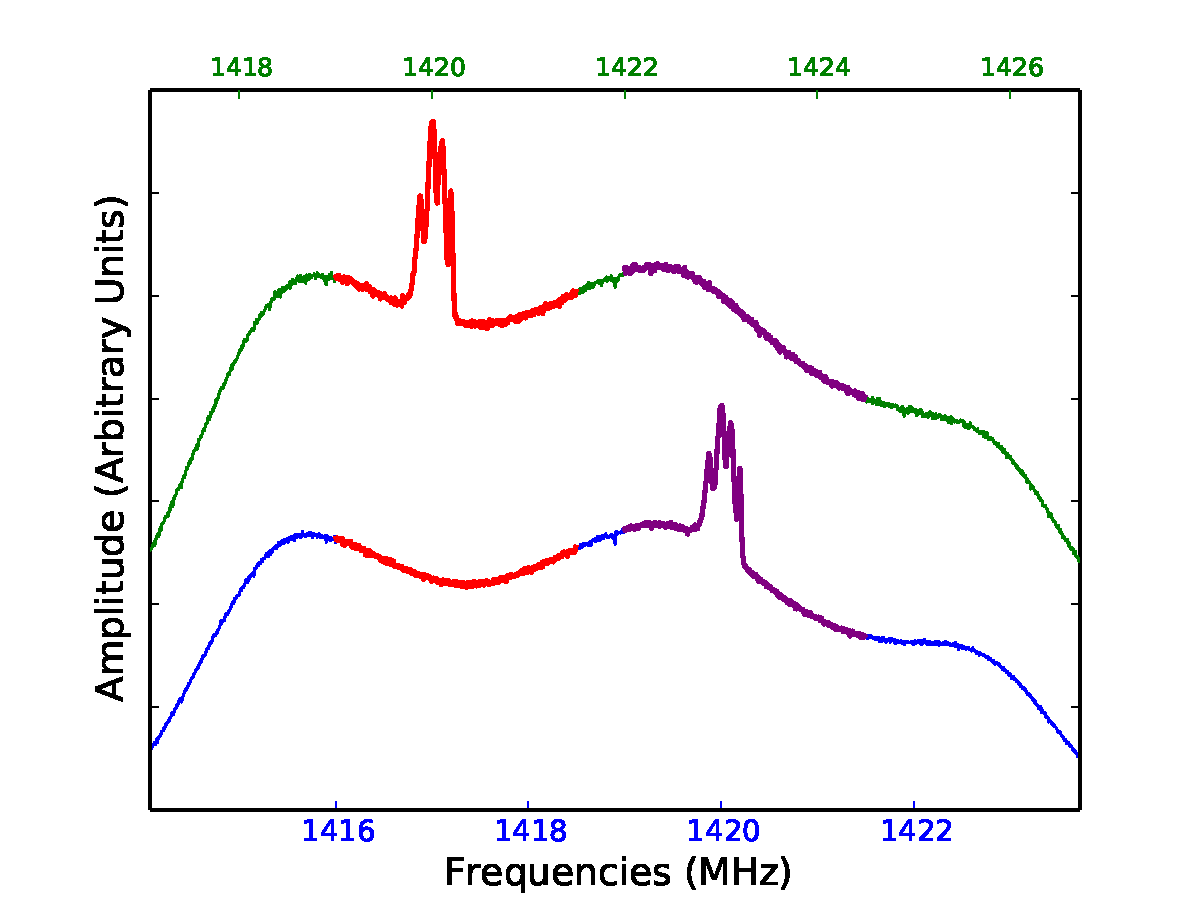
\includegraphics[width=0.5\textwidth]{Excized_Regions.pdf} \\
    \caption{Excision procedure for system temperature and gain determination.  Red, purple colors indicate region of the spectra that are removed in system temperature calculation.  Same colors (i.e. spectral lines) are used to make a first pass at subtracting bandpass gain shape.  Image is courtesy of C. Levy.}
    \label{fig:excized}
\end{figure}

I wrote out the math for this procedure some time ago and it makes sense qualitatively, but Caleb's procedure is slightly different -- it seems as if we compute the system temperature once for each set of spectra, and gain for left/right spectra.



Finally, in order to combine the left and right spectra, I averaged together BOTH the temperatures AND the frequencies of the data for the arrays corresponding the high and low Local Oscillator frequencies. As the indices for each frequency are different, I thought this was a good compromise; this does produce errors of order 10 khz however, so it is possible that this biases our data one way or another if the RF spikes have a systematic patter to them. It would probably be worth discussing this.
-- CALEB

\subsection{Error analysis}

Integration times were chosen so error would be nice (mainly for noise).  Integration time for main observations dictated by physical brightness temp.

I chose the time for noise diode integration so that the error (which arises from a sum/average over all channels) would be order $10\%$ of the channel-by-channel error.

The signal error is calculated as
\[
    5
\]

Output frequency range is $1419$ to $1421.5\unit{MHz}$

% =============
% Data analysis
% =============
\section{Data analysis}

\subsection{Baseline removal and peak identification}

Due to a shortage of time, I did not finish my own
velocity computation etc... scripts.  Mainly needed baseline fitting/removal, peak identification.  (but, after baseline removal, I'd be able to get the main science done).  Working on it now would require branching Isaac's pipeline, and risk messing up the current data processing pipeline.  So I shan't do that yet...

Later on, I really want to be able to decompose the various peaks.  It
looks like our spur observations don't have multiple peaks anyways, so it's not
so bad since we don't care about the galactic plane.

\subsection{$n$-th moment computation}

\subsection{Data interpolation and projection}



% =====================
% Results, pretty image
% =====================
\section{Results}

\subsection{Maps of the North Polar Spur}

\begin{figure}[!ht]
    \centering
    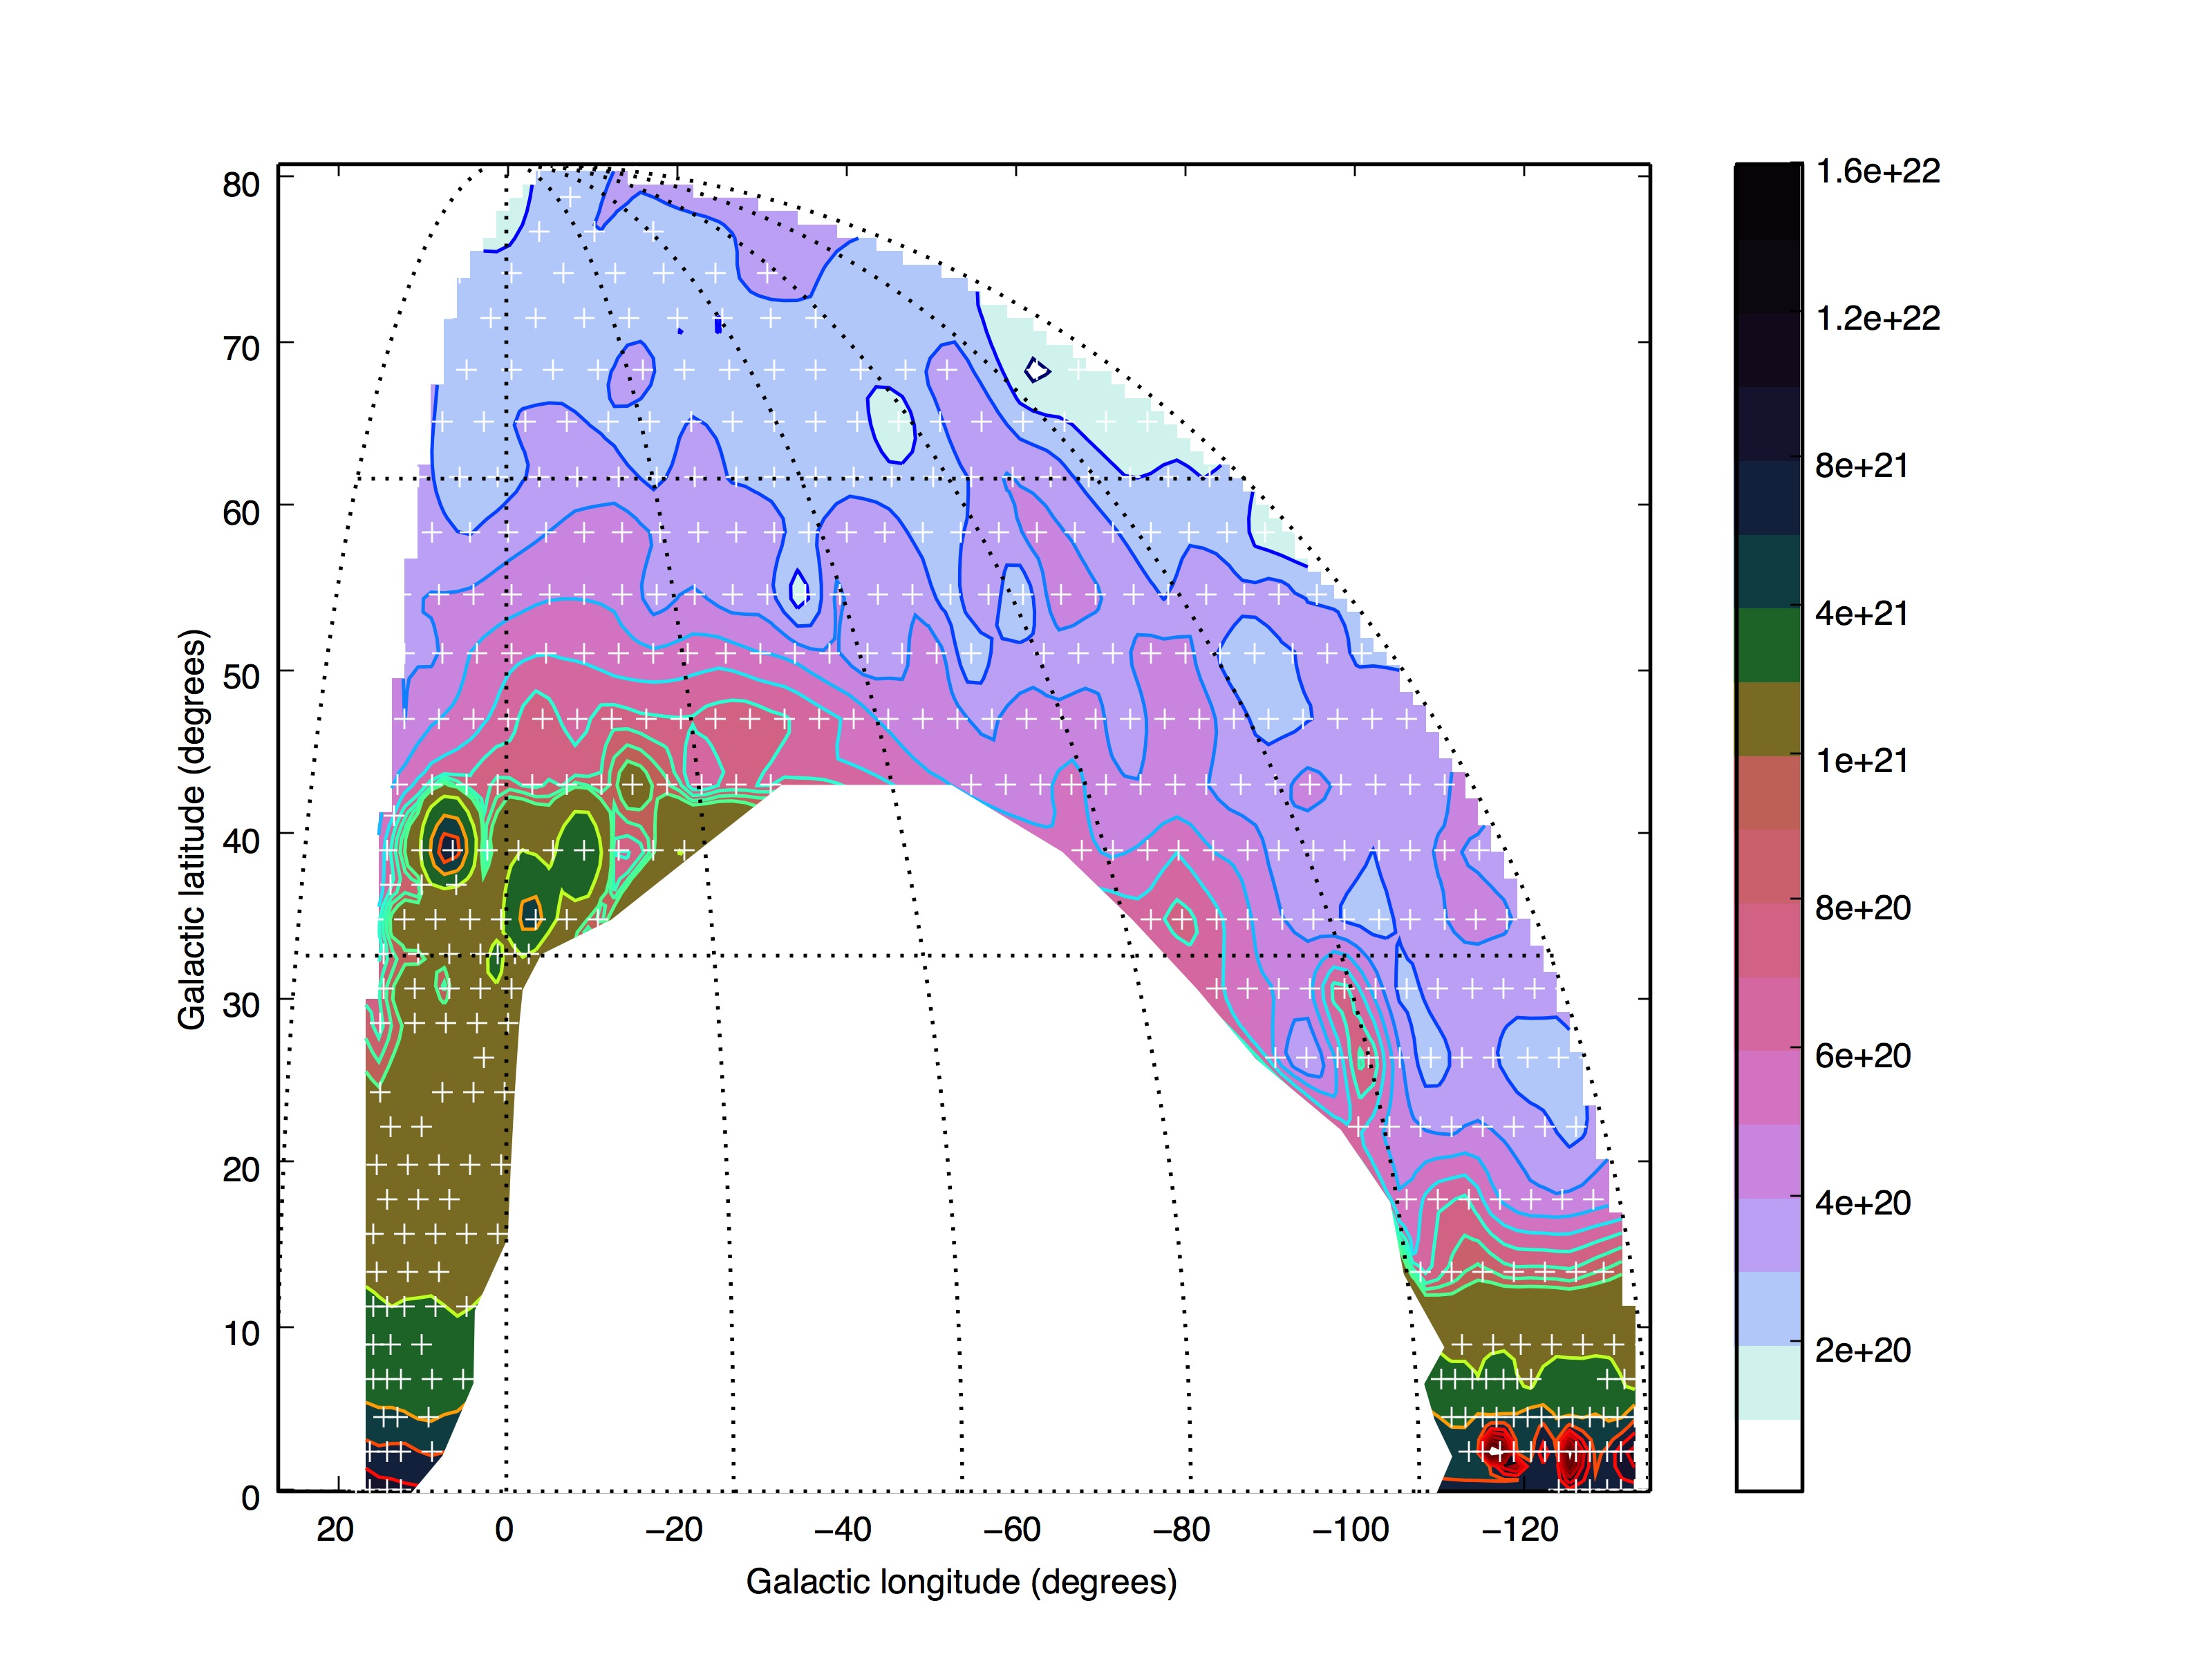
\includegraphics[width=0.5\textwidth]{plots/col_density.jpg} \\
    \caption{Column density.  Note that this is very roughly log scaled.}
    \label{fig:colrho}
\end{figure}
\begin{figure}[!ht]
    \centering
    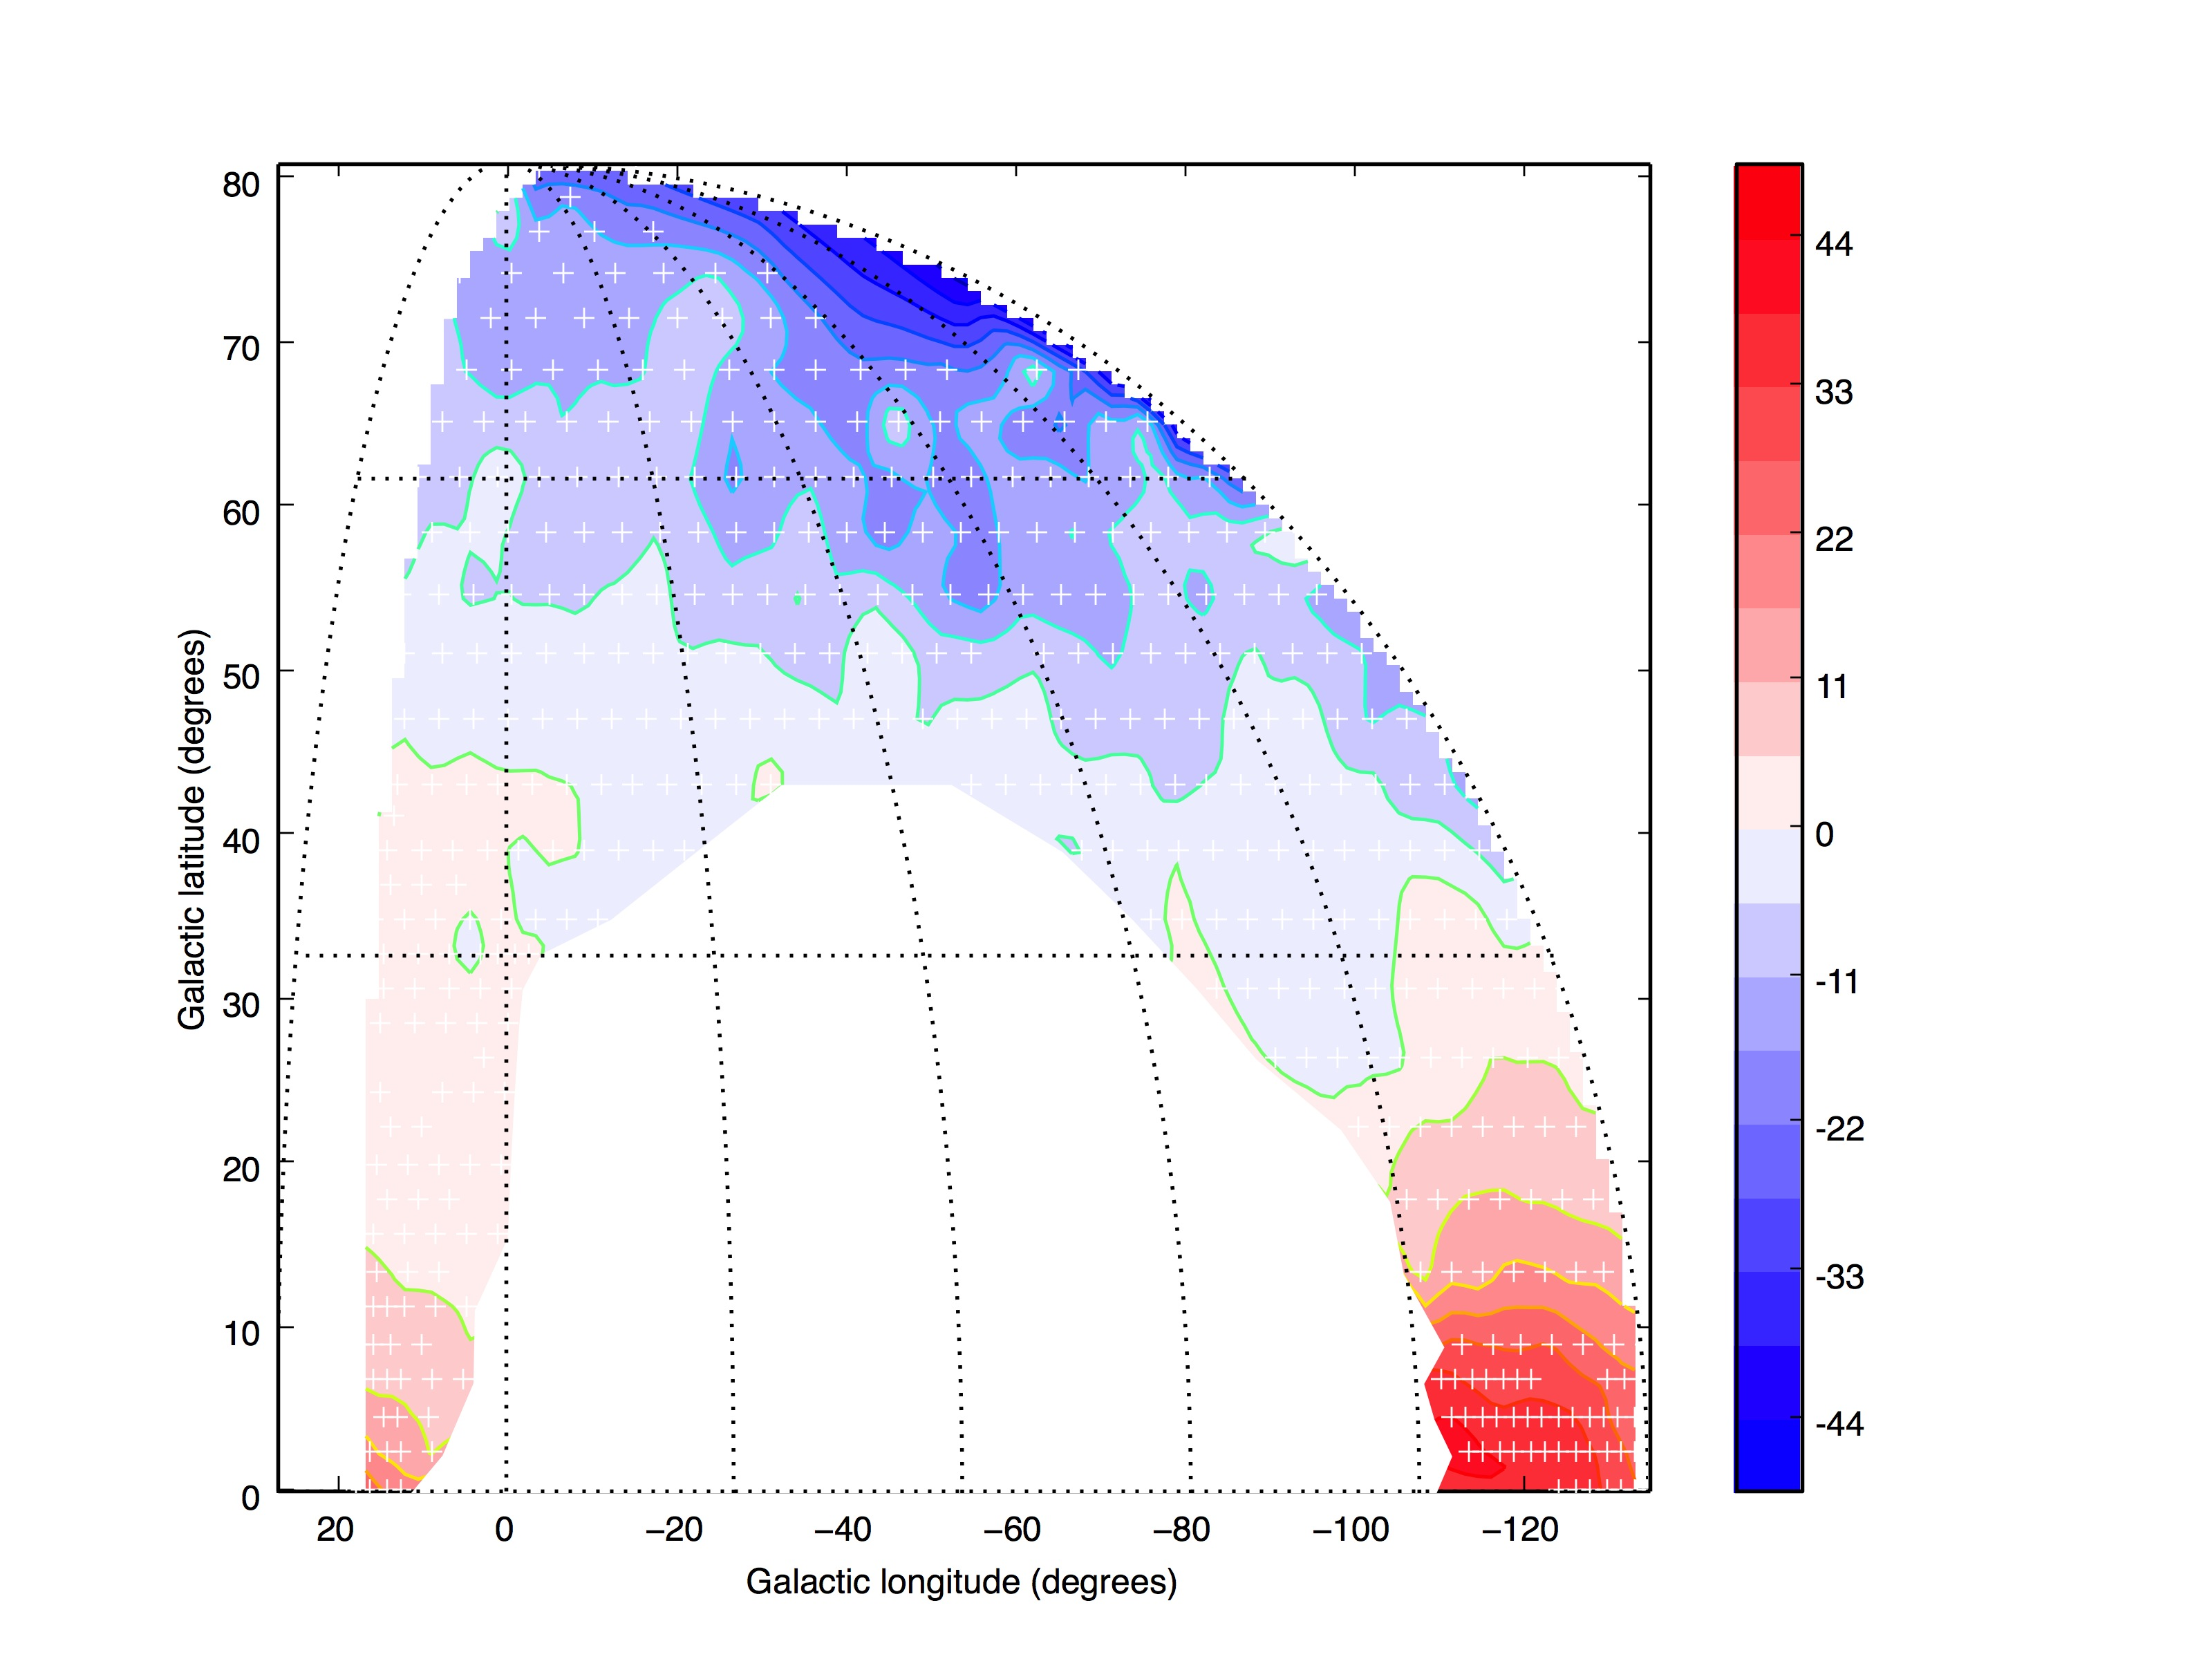
\includegraphics[width=0.48\textwidth]{plots/veloc_mean.jpg}
    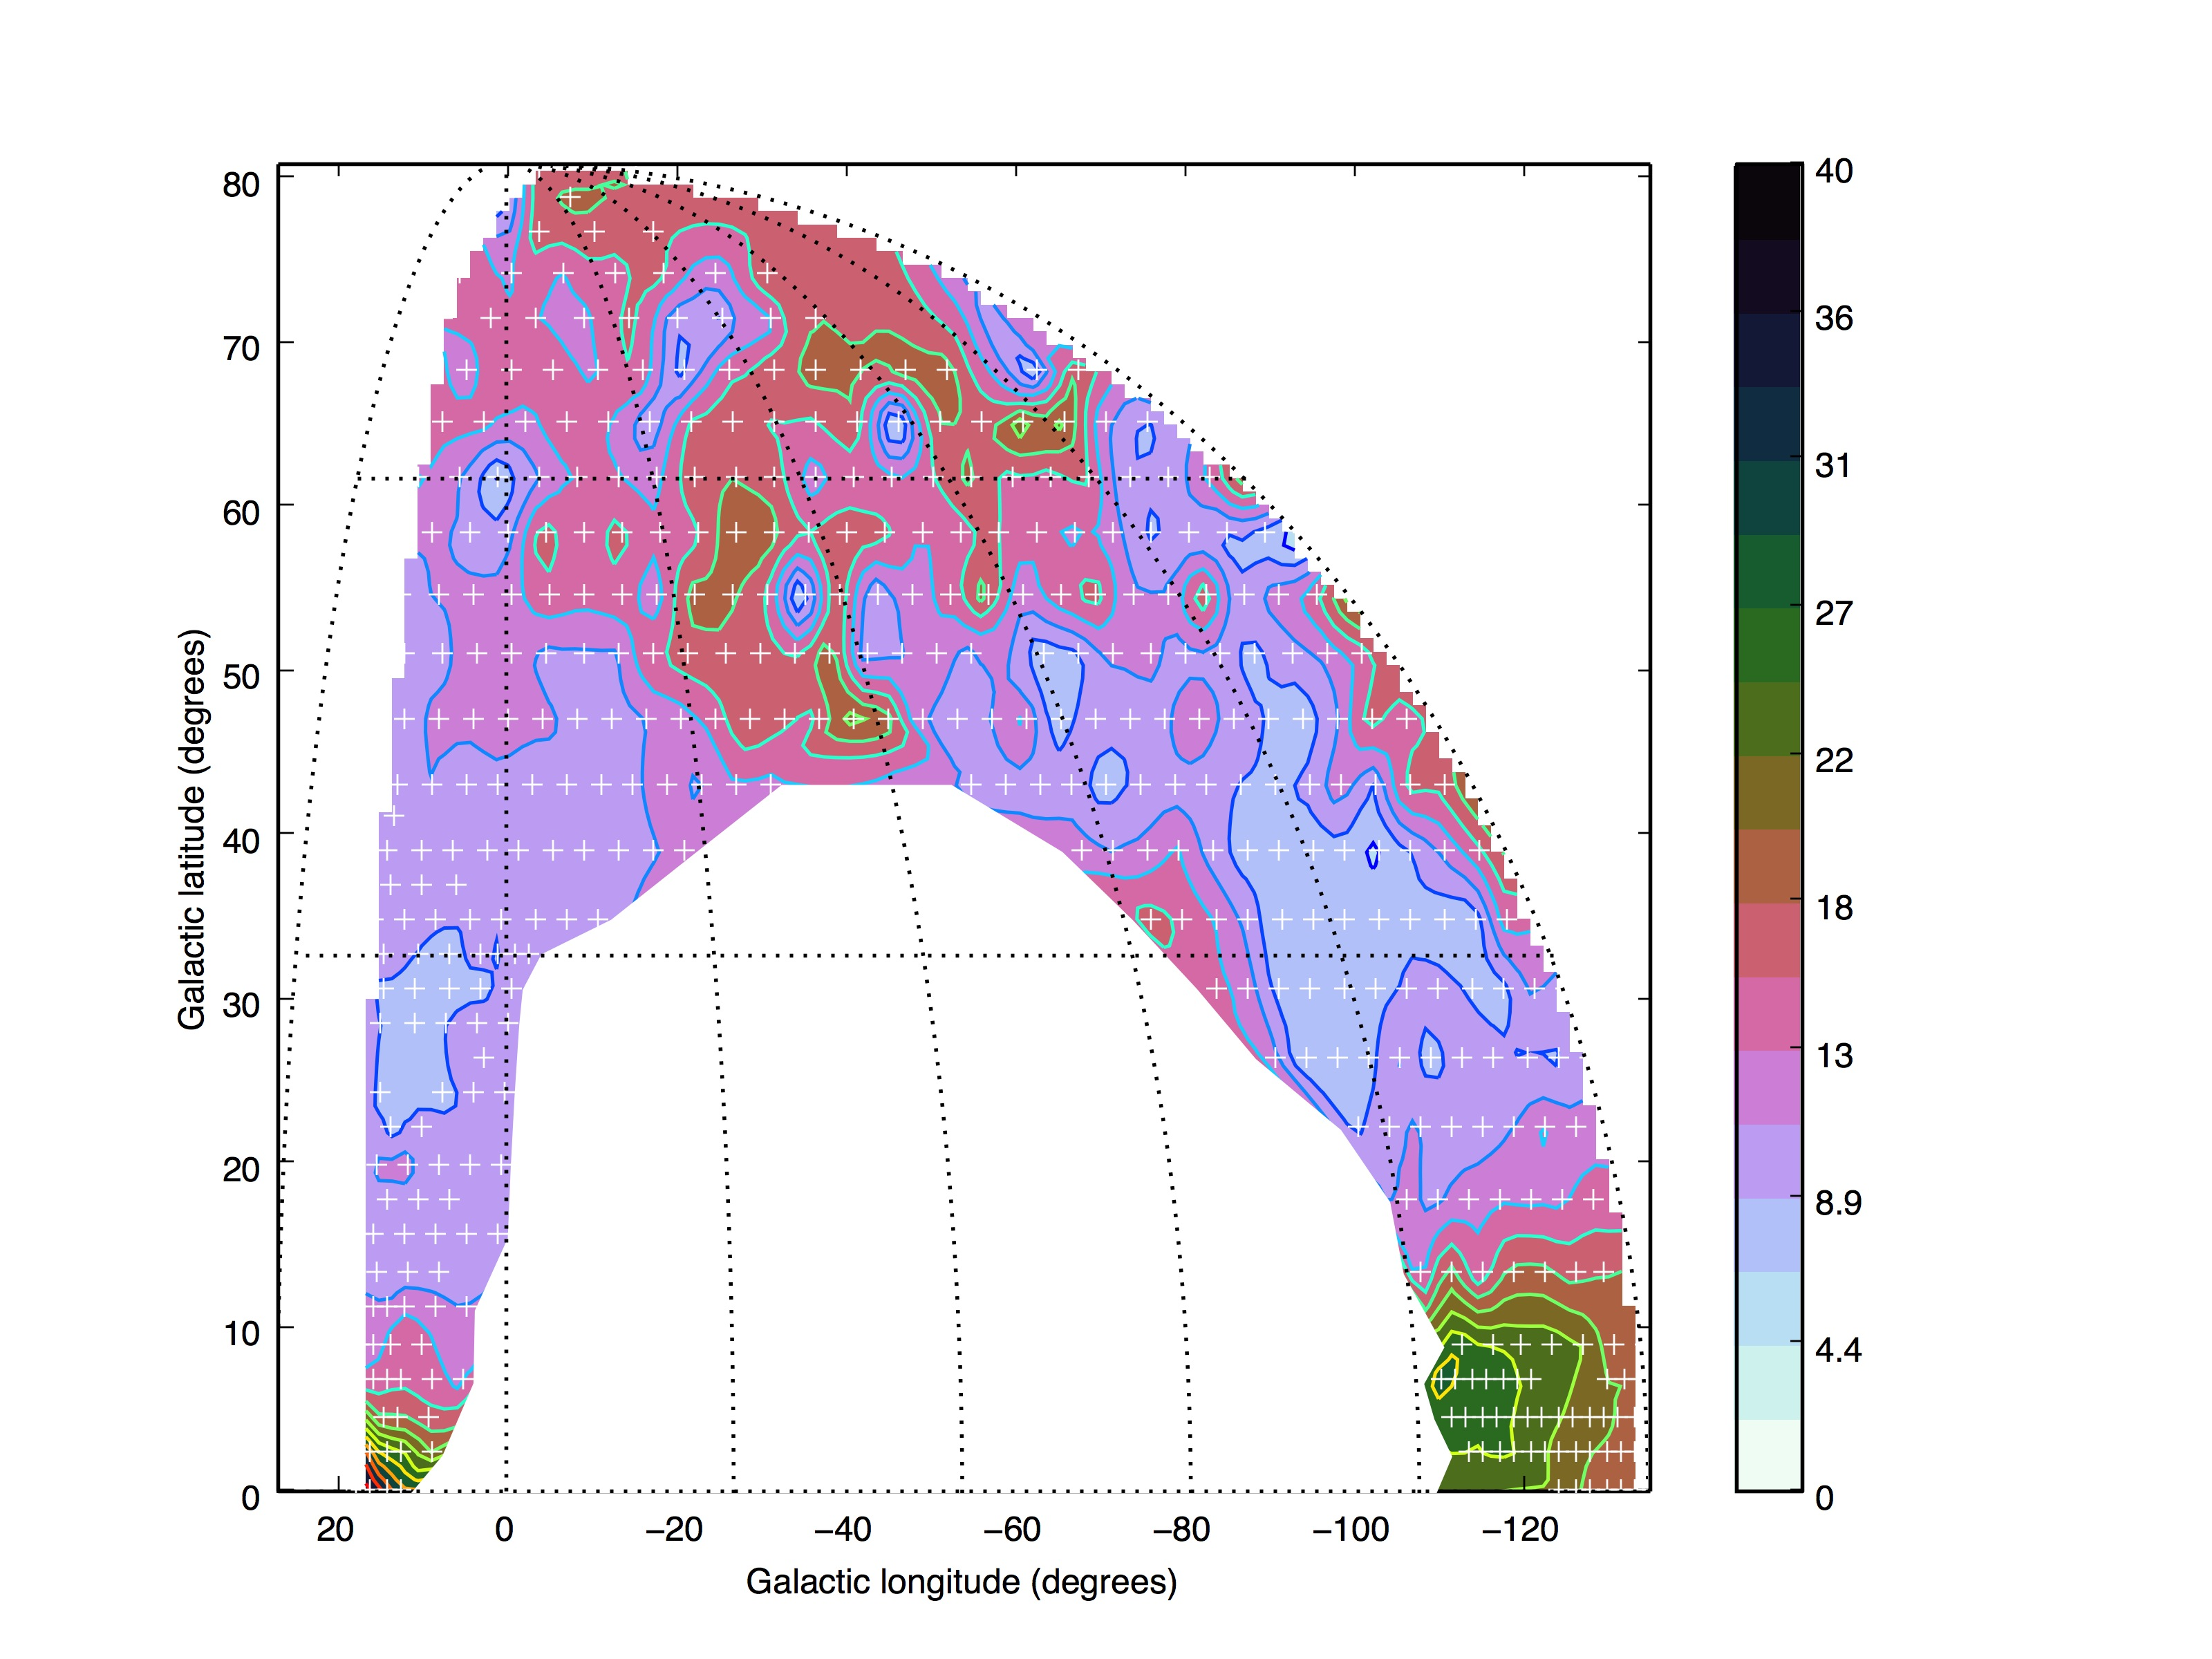
\includegraphics[width=0.48\textwidth]{plots/veloc_std.jpg} \\
    \caption{Mean velocity (left), stdev of velocity (right)}
    \label{fig:velocs}
\end{figure}

Things to do:
\begin{itemize}
    \item Manually compute Gaussian image interpolation
    \item Apply NaN mask to make imshow/contour/contourf plots better (instead of using a polygon to mask unmapped region).  Maybe finish implementing signed distance function here to map out non-rectangular plot domain.
    \item Compare imshow/contour vs. contourf/contour.  Imshow is continuous, technically carries more information.
    \item Consider conformal (stereographic), orthographic projections.    Possibly include multiple images to replicate what a ground observer might see.
    \item Since we are not doing a complete sky map (which is what Mollweide is commonly used for), does there exist a more appropriate equal-area projection? Sinusoidal, Hammer, Aitoff, etc.
    \item Test colormaps in a systematic way.  Determine physiologically sensible colormaps (i.e. no rainbows, jets)
    \item Determine best nonlinear colormapping for column density (logarithmic, power law).  Maybe look at histogram and find the most ``histogram-equalizing'' transformation.
    \item Reduce the load times for both png and pdf... they're really slow.  Maybe I should resort to jpg (welp, ugly, no)
    \item Multiple dimensions in color image -- encode velocity (hue) and column density (brightness) together, with column density nonlinearly scaled.
\end{itemize}

\subsection{Qualitative features}

Comparing the dispersion to the velocity mean looks promising!  As we might expect, dispersion is stronger towards the center of our postulated/expected bubble, a more robust velocity signal is seen at edges.

% ==========
% Discussion
% ==========
\section{Discussion}

\subsection{Physical interpretation of observations}

IF I separate out lines and get individual linewidths etc (by gaussian fit, dispersion for indiv peaks, however you like) -- start considering physical phenomena that give rise to broadening.

Comparison, if there is time: download 1.4 GHz survey data from skyview.gsfc.nasa.gov and generate a comparison plot with same/similar projection.

\subsection{Data reduction biases}

RFI removal and calibration, and spectrum processing, naturally introduces biases.  To remove RFI, we binned the frequency channels into groups of four and took the minimum value in each bin.  Although this kills spikes, this also systematically biases our data downwards, particularly the channel readings where the HI line is present.  We identify the selected bins with the ORIGINAL, ACTUAL frequency tied to that channel (so, the shape is roughly preserved, but the very peaks may be lost).  We also introduce a more uneven frequency spacing and are throwing away data -- this may increase error, although compared to the error of missing an RFI spike this may be a reasonable trade-off!

Caleb's procedure of throwing away 200 pts at edges of spectra -- again, we are losing some (relatively unimportant) information.  But, it helps cut down noise in the summation (more integration time, after a fashion).

\subsection{RFI mitigation}

Radio frequency interference was not actively characterized and addressed in this study.  We suggest several approaches to addressing RFI in future work.

The quantity of interference signal is highly variable, with some spectra slathered in spikes and other spectra relatively unaffected.  We speculate there may be multiple explanations.  (1) geostationary satellites at fixed az-alt may contaminate certain pointings -- this could be mitigated with prior knowledge of satellite az/alt. (2) airplanes.  (3) if the RFI is from ground based transmission -- e.g. if there are fewer transmissions at a certain time of day, or there is a directional dependence to broadcasts (wherever radio towers are located).

(if there is time -- supply az,alt,time of pointings)
(it would be nice to create a measure of how much RFI is present, then plot against az,alt to see if there is a portion of the sky that is particularly susceptible to contamination.  We could do this with just our data for an incomplete, uneven survey, but it would be something.)
(and, also plot the temporal dependance)

Tabulate list of sources
https://casper.berkeley.edu/wiki/images/8/82/RPA5.pdf, see also VLA lists for examples.

Any future all-sky survey undertaken with the leuschner dish in May might want to map this region of the sky, then write the dish tracking script to avoid it.  also keep track of where the sun and moon are.

If there is any way to probe polarization (as it seems they were once able to do with the RPA interferometer), we might be able to identify signals with strong polarization as being affiliated with human transmission [\textit{Harp and Ackerman}, 2001].

% ===========
% Conclusions
% ===========
\section{Conclusions}

Pretty pictures are gr8.

\section{Appendix A: rainbow colormap considered harmful}

Comparison plots for different colormaps.

\begin{figure}[!ht]
    \centering
    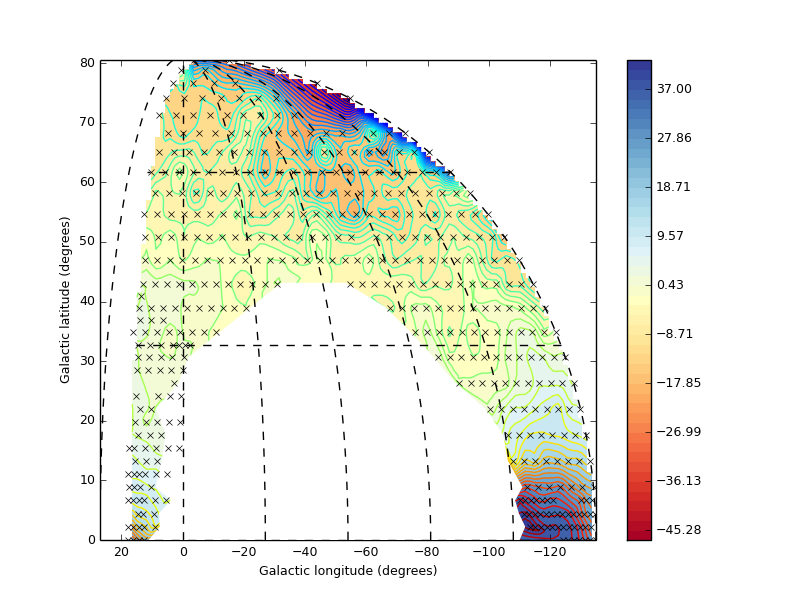
\includegraphics[width=0.48\textwidth]{v_ave_temporary.png}
    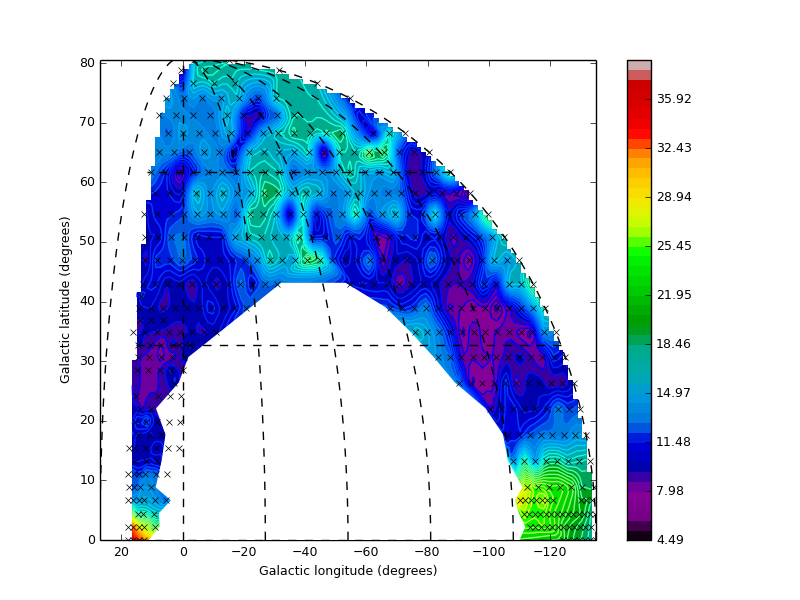
\includegraphics[width=0.48\textwidth]{v_std_temporary.png} \\
    \caption{Mean velocity (left), stdev of velocity (right).  Units are km/s for colors.}
    \label{fig:velocs_again}
\end{figure}

They look so pretty... but they're not as meaningful as they seem.

% ===============
% Acknowledgments
% ===============
\section{Acknowledgments}

\begin{figure}[!ht]
    \centering
    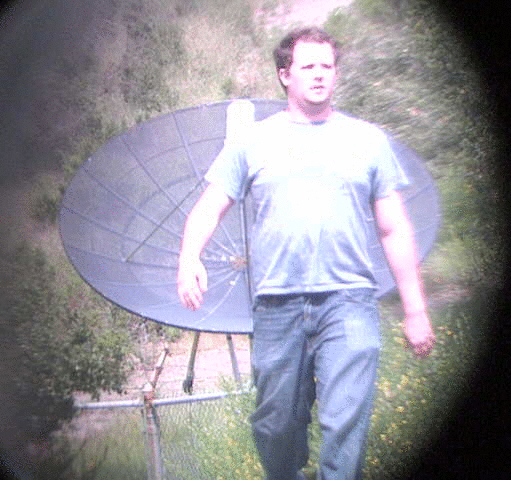
\includegraphics[width=0.5\textwidth]{kartp2.png} \\
    \caption{(image courtesy of I. Domagalski, E. Herrera, K. Moses)}
    \label{fig:kartp2}
\end{figure}

\begin{center}
Kartp noster, qui es in radiolab:\\
sanctificetur nomen tuum;\\
adveniat regnum tuum;\\
fiat voluntas tua.\\
sicut in academia, et in universitas.\\
Observationem nostrum cotidianum da nobis hodie;\\
et dimitte nobis errores nostra,\\
sicut et nos dimittimus erroribus nostris;\\
et ne nos inducas in tentationem;\\
sed libera nos a circumsonum.
\end{center}

Five pieces of duct tape.

%Karto and Baylee are gr8.
%Isaac and Caleb are gr8.
%Aaron Parsons is cool.

\section{Author contributions}

I. A. D. did almost everything tracking.  C. L. did all calibration.  A. T. did some of the tracking.  All parties contributed to debugging.

\section{Electronic supplement}

All supporting files are stored on the repository:\\
\href{https://github.com/aarontran/ay121}
{https://github.com/aarontran/ay121/lab4/}.

\section{References}

\hangindent 0.25in Condon, J. J. and S. M. Ransom (2006), Essential Radio Astronomy, \\
\href{http://www.cv.nrao.edu/course/astr534/ERA.shtml}
{http://www.cv.nrao.edu/course/astr534/ERA.shtml}.

\hangindent 0.25in Green, R. M. (1985), \textit{Spherical astronomy}, 520pp.,
Cambridge Univ. Press, Cambridge.

\hangindent 0.25in Harp, G. R. and R. F. Ackermann (2001), RFI Survey at the RPA, \\ \href{https://casper.berkeley.edu/wiki/images/f/f9/RPA11.pdf}{https://casper.berkeley.edu/wiki/images/f/f9/RPA11.pdf}.

\hangindent 0.25in Heiles, C., Y.-H. Chu, R. J. Reynolds, I. Yegingil, and T. H. Troland (1980), A new look at the North Polar Spur, \textit{Astrophys. J.}, \textit{242}, 533--540, doi:10.1086/158487.

\hangindent 0.25in Siemion, A. (2012), Leuschner Spectrometer, CASPER documentation wiki, \\
\href{https://casper.berkeley.edu/wiki/Leuschner\_Spectrometer}
{https://casper.berkeley.edu/wiki/Leuschner\_Spectrometer}.

\hangindent 0.25in Wolleben, M. (2007), A New Model for the Loop I (North Polar
Spur) Region, \textit{Astrophys. J.}, \textit{664}, 349--356,
doi:10.1086/518711.

\end{document}
